\chapter{Neural Calibration as an Inverse Problem}
\label{ch:cann}

The previous chapter asked whether a neural network can reproduce the Heston implied-volatility map with sufficient accuracy to be useful as a pricer. This chapter turns the direction of the question around. Given a finite implied-volatility surface, what Heston parameter vector is implied by it, and how much confidence should be attached to that answer?

This change of direction is important. Pricing is a forward approximation problem: the parameters and contract descriptors are known, and the network returns an implied volatility. Calibration is an inverse problem: the surface is observed, while the parameter vector
\[
\theta=(\rho,\kappa,\gamma,\bar v,v_0)
\]
must be inferred. The same ANN pricer is therefore used in a different role. It is no longer the object being trained, but a fixed computational instrument inside an optimization loop.

The calibration strategy follows the neural calibration framework of Liu et al. \cite{liu}. The inherited principle is to avoid repeated calls to a full Heston pricing engine during calibration. Instead, a trained ANN forward surrogate is frozen and used to evaluate candidate Heston parameters quickly in implied-volatility space. The implementation in this thesis keeps this principle, but treats the output of the calibration stage as something that must be inspected rather than merely reported. Residual maps, regularization checks, and local curvature diagnostics are therefore part of the method, not only of the final benchmark.

The narrative of this chapter is consequently diagnostic. First, the inverse problem is defined in the same variables used by the ANN pricer. Second, the numerical calibration loop is described. Third, the chapter explains how the resulting optimum is audited: does it fit the surface, is the solution locally stable, and which parameters are strongly or weakly identified by the available quotes? The detailed benchmark numbers are reported in Chapter~\ref{ch:performance_benchmarks}; here the focus is the calibration mechanism and the evidence required to interpret it.

\begin{figure}[H]
    \centering
    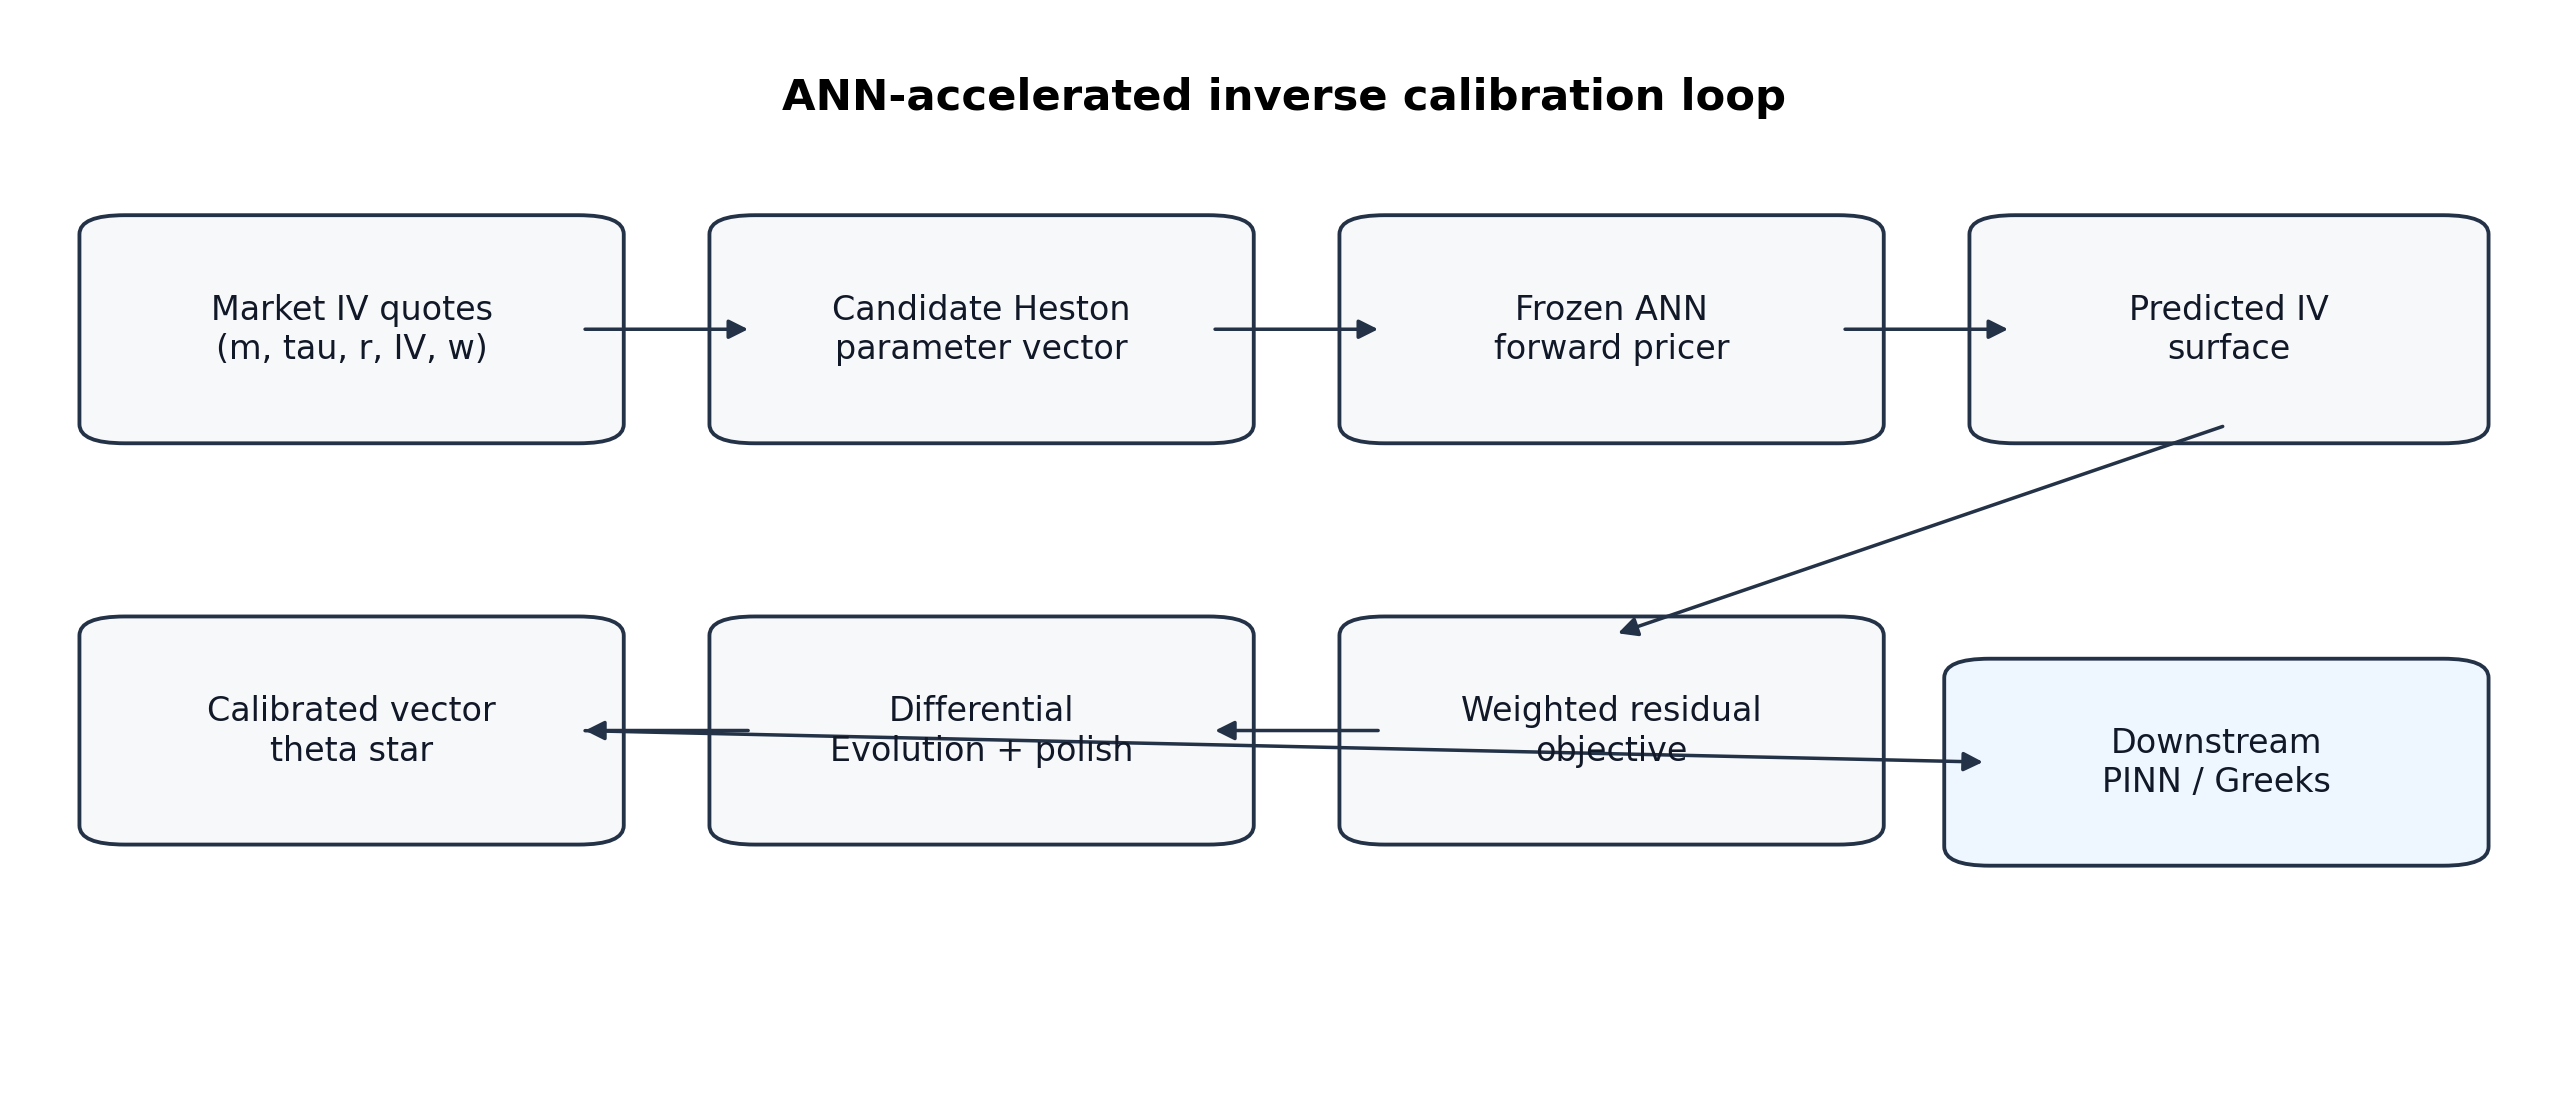
\includegraphics[width=0.98\textwidth]{figures/cann/cann_workflow_diagram.png}
    \caption{ANN-accelerated inverse calibration workflow. Market implied-volatility quotes are compared with ANN-implied surfaces generated from candidate Heston vectors, and Differential Evolution searches for the vector that minimizes the weighted residual objective.}
    \label{fig:cann_workflow}
\end{figure}

%%%%%%%%%%%%%%%%%%%%%%%%%%%%%%%%%%%%%%%%%%%%%%%%%
\section{From Forward Pricing to Inverse Calibration}

The ANN surrogate trained in Chapter~\ref{ch:ann_surrogate} approximates the forward map
\[
f_{NN}:(\rho,\kappa,\gamma,\bar v,v_0,m,\tau,r)\mapsto \sigma_{\mathrm{IV}},
\]
where \(m=S_0/K\), \(\tau=T-t\), and \(\sigma_{\mathrm{IV}}\) is the implied volatility returned by the numerical Heston-COS/Brent pipeline during training.

Calibration uses this map as an inner evaluator. For each candidate \(\theta\), the quote grid is completed with the repeated Heston parameters, passed through the frozen ANN, and compared with the observed implied-volatility surface. The optimizer never sees the true parameter vector in the synthetic experiment. It only sees the quote table, the admissible bounds, and the residual objective.

This distinction makes the stage more than a speed-up device. A small residual means that the candidate vector reproduces the quoted surface well on the available grid. It does not automatically mean that each component of \(\theta\) has been uniquely recovered. Heston parameters can compensate for one another over a finite set of maturities and strikes, especially when the quote surface is smooth and sparse. For that reason, calibration quality is evaluated at two levels throughout the thesis: fit quality in implied-volatility space and parameter identifiability around the selected optimum.

The output of this chapter is also the input to the later PINN workflow. Once the calibrated vector
\[
\theta^\star=(\rho^\star,\kappa^\star,\gamma^\star,\bar v^\star,v_0^\star)
\]
has been obtained, the structural parameters \((\rho^\star,\kappa^\star,\gamma^\star,\bar v^\star)\) define the Heston operator used by the downstream pricing model, while \(v_0^\star\) fixes the current variance state at market evaluation time.

%%%%%%%%%%%%%%%%%%%%%%%%%%%%%%%%%%%%%%%%%%%%%%%%%
\section{Calibration Surface and Quote Encoding}

The calibration surface is represented as a finite quote table
\[
\mathcal{Q}=\{(m_j,\tau_j,r_j,\sigma^{\mathrm{mkt}}_j,w_j)\}_{j=1}^{N_q},
\]
where \(w_j\geq 0\) is an optional quote weight. This representation is intentionally close to the input format used by the ANN pricer. The model does not require the quote grid to be rectangular, although the benchmark experiment uses a complete grid to make the residual and curvature diagnostics easier to read.

\begin{table}[H]
    \ttabbox[\FBwidth]
    {\caption{Quote-table representation used in calibration.}\label{tab:cann_quote_columns}}
    {\begin{tabular}{|P{3.0cm}|P{8.7cm}|}
        \hline
        \textbf{Column} & \textbf{Meaning} \\
        \hline
        \texttt{moneyness} & \(m=S_0/K\), with the same convention as the ANN pricer. \\
        \hline
        \texttt{tau} & Time to maturity \(\tau=T-t\). \\
        \hline
        \texttt{r} & Risk-free rate associated with the quote. \\
        \hline
        \texttt{iv\_market} & Observed or synthetic market implied volatility. \\
        \hline
        \texttt{weight} & Quote weight used in the calibration objective; unit weights are used if absent. \\
        \hline
        \multicolumn{2}{l}{Source: Own calibration pipeline.}
    \end{tabular}}
\end{table}

The benchmark quote universe contains \(35\) contracts arranged over five moneyness nodes and seven maturities. Figure~\ref{fig:cann_quote_surface} shows the surface used as calibration input. The figure is useful because it fixes the information content of the inverse problem: only this discrete surface is available to the optimizer.

\begin{figure}[H]
    \centering
    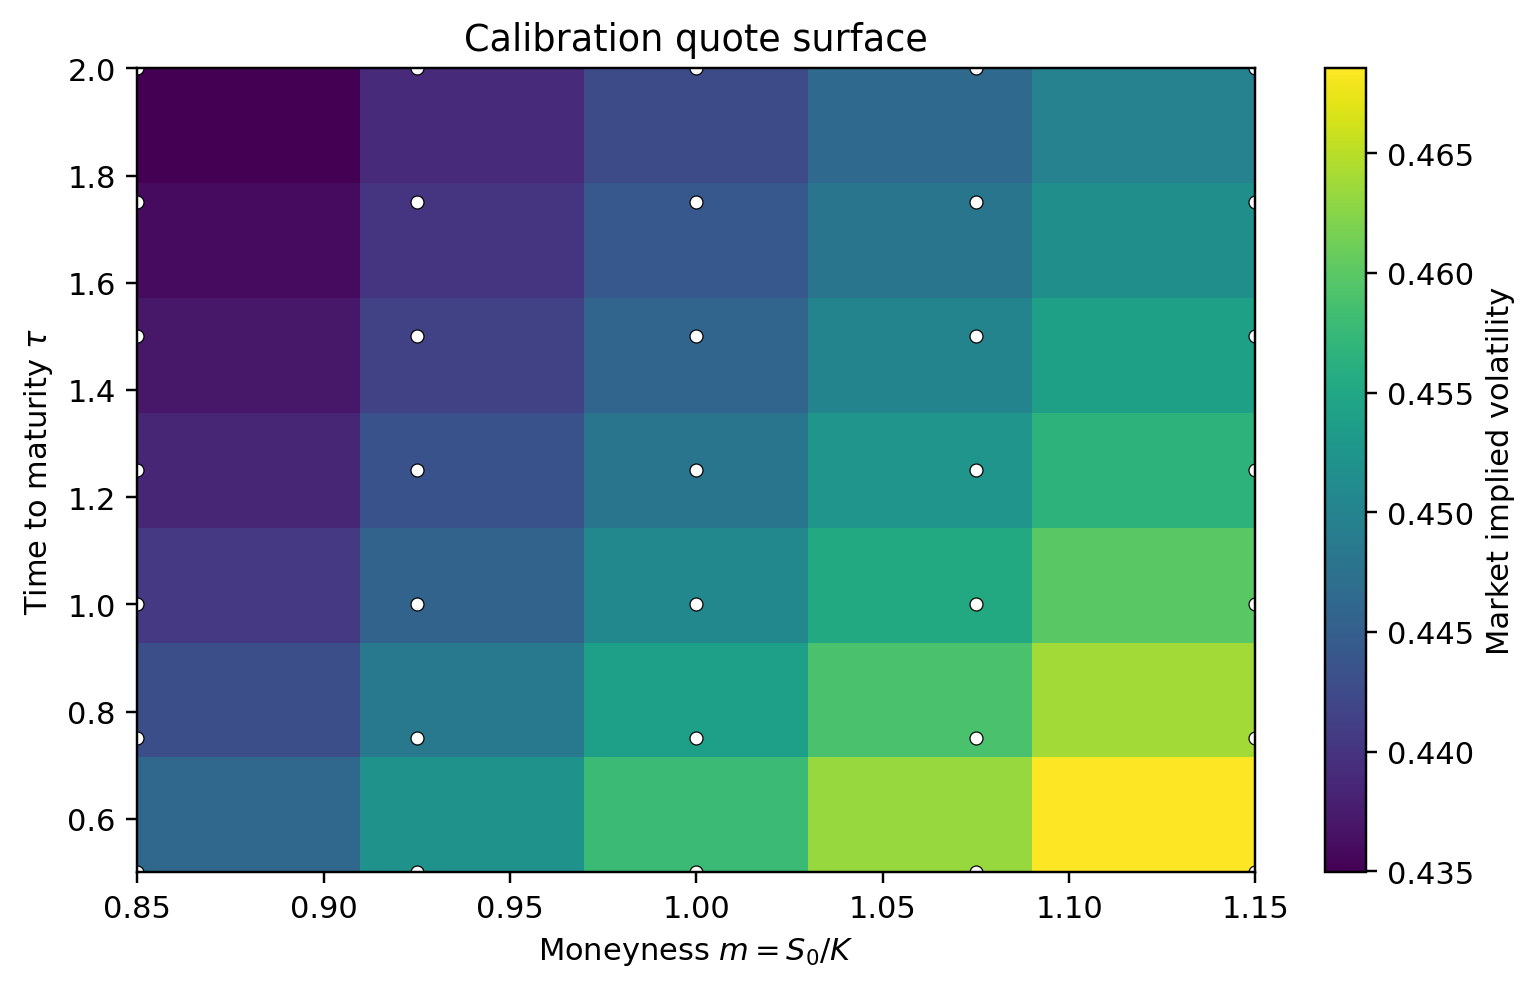
\includegraphics[width=0.82\textwidth]{figures/cann/cann_quote_surface.png}
    \caption{Implied-volatility surface used as calibration input in the Liu-style synthetic experiment. Markers show the \(35\) observed quote locations.}
    \label{fig:cann_quote_surface}
\end{figure}

For a fixed candidate \(\theta\), the implementation constructs the ANN input matrix
\[
X(\theta)=
\begin{bmatrix}
\rho & \kappa & \gamma & \bar v & v_0 & m_1 & \tau_1 & r_1\\
\rho & \kappa & \gamma & \bar v & v_0 & m_2 & \tau_2 & r_2\\
\vdots & \vdots & \vdots & \vdots & \vdots & \vdots & \vdots & \vdots\\
\rho & \kappa & \gamma & \bar v & v_0 & m_{N_q} & \tau_{N_q} & r_{N_q}
\end{bmatrix}.
\]
The Heston parameters are constant across rows, while the contract descriptors vary by quote. This construction keeps calibration aligned with the supervised pricer: no new feature convention is introduced at the inverse stage.

%%%%%%%%%%%%%%%%%%%%%%%%%%%%%%%%%%%%%%%%%%%%%%%%%
\section{Objective Function and Bounds}

For each quote \(j\), the ANN prediction under candidate \(\theta\) is
\[
\hat\sigma_j(\theta)
=f_{NN}(\rho,\kappa,\gamma,\bar v,v_0,m_j,\tau_j,r_j),
\qquad j=1,\dots,N_q,
\]
and the residual is
\[
e_j(\theta)=\hat\sigma_j(\theta)-\sigma^{\mathrm{mkt}}_j.
\]
Calibration is performed in implied-volatility space. This is consistent with Liu et al. \cite{liu}, with the ANN training target, and with the market convention used to compare smiles across strikes and maturities. It also avoids raw price scale effects that would otherwise mix moneyness, discounting, maturity, and payoff magnitude.

The objective minimized in the calibration loop is
\begin{equation}
\label{eq:cann_objective}
J(\theta)
=
\frac{1}{\sum_{j=1}^{N_q} w_j}
\sum_{j=1}^{N_q} w_j e_j(\theta)^2
+\lambda R(\theta).
\end{equation}
The implementation can evaluate the unnormalized weighted sum inside the optimizer; when \(\lambda=0\), this differs only by a positive constant factor and therefore has the same minimizer. Reported metrics in Chapter~\ref{ch:performance_benchmarks} use the normalized weighted-MSE convention.

The calibrated vector is
\begin{equation}
\label{eq:cann_argmin}
\theta^\star
=
\arg\min_{\theta\in\mathcal{B}}J(\theta),
\end{equation}
where \(\mathcal{B}\) is the admissible Heston parameter box. The bounds used in this stage are shown in Table~\ref{tab:cann_parameter_bounds}.

\begin{table}[H]
    \ttabbox[\FBwidth]
    {\caption{Calibration parameter bounds used in the CaNN stage.}\label{tab:cann_parameter_bounds}}
    {\begin{tabular}{|P{3.0cm}|P{4.5cm}|P{4.5cm}|}
        \hline
        \textbf{Parameter} & \textbf{Lower bound} & \textbf{Upper bound} \\
        \hline
        \(\rho\) & \(-0.9\) & \(0.0\) \\
        \hline
        \(\kappa\) & \(0.0\) & \(3.0\) \\
        \hline
        \(\gamma\) & \(0.01\) & \(0.8\) \\
        \hline
        \(\bar v\) & \(0.01\) & \(0.5\) \\
        \hline
        \(v_0\) & \(0.05\) & \(0.5\) \\
        \hline
        \multicolumn{3}{l}{Source: Own configuration, aligned with the ANN training domain.}
    \end{tabular}}
\end{table}

The bounds have a methodological role. They define the region in which the Heston parameters are considered admissible for this thesis, and they restrict the optimizer to the interpolation regime of the ANN pricer. Without this restriction, the calibration loop could exploit extrapolation artifacts of the surrogate rather than fitting the Heston model in a meaningful domain.

%%%%%%%%%%%%%%%%%%%%%%%%%%%%%%%%%%%%%%%%%%%%%%%%%
\section{Batched Calibration Architecture}

The calibration architecture is a composition of three elements: a frozen ANN pricer, a quote encoder, and a global optimizer. This differs from training a direct inverse network from surfaces to parameters. A direct inverse network would be extremely fast once trained, but it would require a separate supervised dataset of volatility surfaces and known parameter vectors. In the present thesis, the inverse problem is solved explicitly for the observed quote set, which makes the objective, residuals, and optimizer diagnostics directly inspectable.

For a population of \(S\) candidate vectors,
\[
\Theta_{\mathrm{pop}}=\{\theta^{(1)},\dots,\theta^{(S)}\},
\]
the implementation evaluates all candidates in vectorized form. The feature matrix contains \(S\times N_q\) rows, the ANN returns \(S\times N_q\) implied-volatility predictions, and the predictions are reshaped into \(S\) surfaces before applying Equation~\eqref{eq:cann_objective}. Figure~\ref{fig:cann_vectorized_evaluation} summarizes this data flow.

\begin{figure}[H]
    \centering
    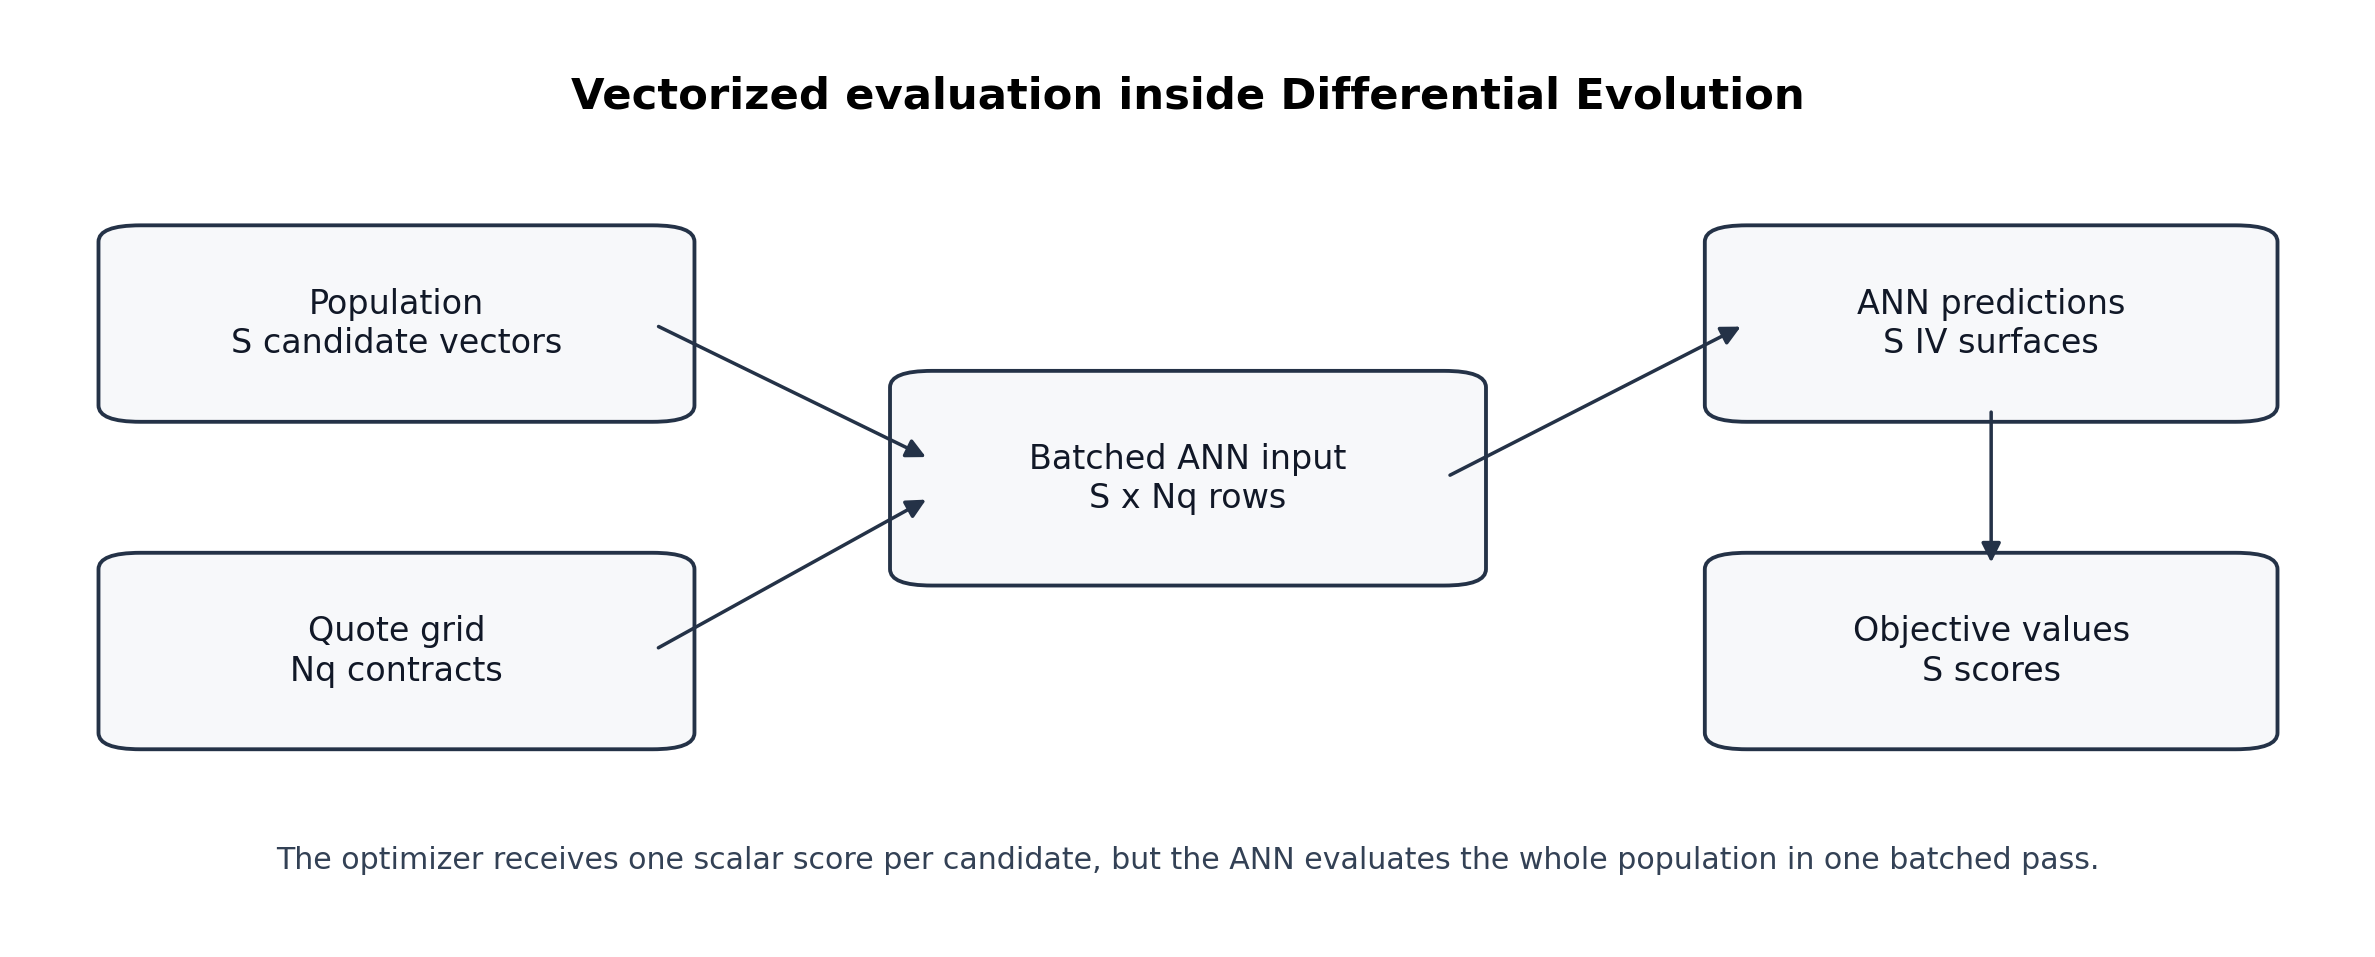
\includegraphics[width=0.92\textwidth]{figures/cann/cann_vectorized_evaluation.png}
    \caption{Vectorized population evaluation used inside the calibration loop. Candidate parameters are crossed with the quote grid, scored as implied-volatility surfaces, and returned to the optimizer as one objective value per candidate.}
    \label{fig:cann_vectorized_evaluation}
\end{figure}

This batching step is not a cosmetic implementation detail. Differential Evolution evaluates many candidates per iteration, and the ANN acceleration is only fully exploited when those evaluations are aggregated into large forward passes. The speed gain is therefore produced by two layers working together: the neural surrogate replaces the numerical Heston solver, and vectorized inference replaces repeated scalar evaluations.

%%%%%%%%%%%%%%%%%%%%%%%%%%%%%%%%%%%%%%%%%%%%%%%%%
\section{Differential Evolution Search}

The inverse residual surface is not assumed to be convex. Several Heston parameter combinations can generate similar implied-volatility smiles over a finite grid, and local methods may depend heavily on the starting point. The baseline optimizer is therefore Differential Evolution (DE), a population-based global optimization method for continuous variables \cite{storn1997de}.

DE maintains a population of candidate vectors inside the admissible bounds. At each iteration, mutation and crossover generate trial vectors. A trial replaces an existing candidate when it improves the objective. The procedure does not require gradients of \(J\), which is useful because the calibrated objective includes a neural surrogate, quote weights, bounds, and optional regularization.

\begin{table}[H]
    \ttabbox[\FBwidth]
    {\caption{Differential Evolution controls used in the calibration pipeline.}\label{tab:cann_de_controls}}
    {\begin{tabular}{|P{4.2cm}|P{7.2cm}|}
        \hline
        \textbf{Control} & \textbf{Value / interpretation} \\
        \hline
        Maximum iterations & \(1000\) \\
        \hline
        Population size multiplier & \(20\), giving an effective population proportional to the number of calibrated parameters. \\
        \hline
        Tolerance & \(10^{-4}\) \\
        \hline
        Mutation range & \([0.5,1.0]\) \\
        \hline
        Recombination & \(0.7\) \\
        \hline
        Polish & Enabled, so the final DE solution can be locally refined. \\
        \hline
        \multicolumn{2}{l}{Source: Own calibration configuration.}
    \end{tabular}}
\end{table}

The advantage of DE is robustness to initialization and multimodality. The cost is the number of objective evaluations. This cost would be prohibitive with a full COS/Brent valuation loop inside each objective call, but it becomes manageable when surface evaluation is reduced to batched ANN inference.

%%%%%%%%%%%%%%%%%%%%%%%%%%%%%%%%%%%%%%%%%%%%%%%%%
\section{Regularization as a Stability Check}

The optional regularization term \(R(\theta)\) in Equation~\eqref{eq:cann_objective} is included to control the inverse problem when the quote set is sparse, noisy, or nearly flat in some parameter directions. The implementation supports no regularization, \(L^1\), \(L^2\), and squared-\(L^2\) penalties:
\[
R_{L^1}(\theta)=\|\theta\|_1,\qquad
R_{L^2}(\theta)=\|\theta\|_2,\qquad
R_{L^2\text{-sq}}(\theta)=\|\theta\|_2^2.
\]

In the synthetic experiment used for the benchmark, the no-regularization run is retained as the reference. Figure~\ref{fig:cann_regularization_rmse} shows that adding a small \(L^2\) penalty changes the residual RMSE only marginally for the selected quote set. This does not make regularization irrelevant. Rather, it indicates that this controlled surface is already sufficiently informative for the reference calibration, while the same interface remains useful for future market-data experiments with bid--ask noise, missing maturities, or uneven liquidity.

\begin{figure}[H]
    \centering
    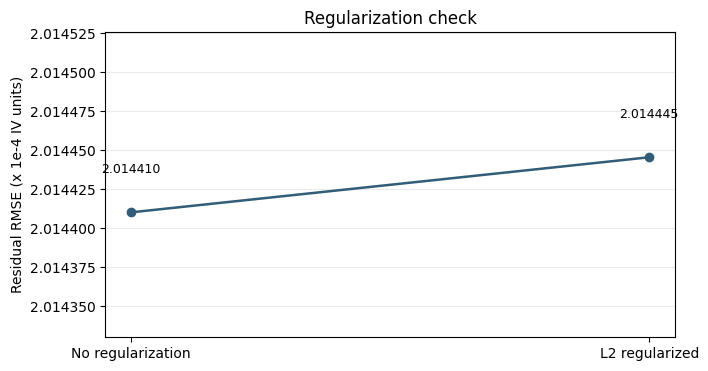
\includegraphics[width=0.72\textwidth]{figures/cann/cann_regularization_rmse.png}
    \caption{Residual RMSE comparison between the no-regularization reference calibration and a small \(L^2\)-regularized variant. The difference is negligible for the controlled synthetic quote set.}
    \label{fig:cann_regularization_rmse}
\end{figure}

Regularization is therefore treated here as a stability probe. If a small penalty moved the optimum substantially while leaving the residual almost unchanged, that would be evidence of weak parameter identification. In the selected run, the main identifiability evidence instead comes from the local curvature analysis described next.

%%%%%%%%%%%%%%%%%%%%%%%%%%%%%%%%%%%%%%%%%%%%%%%%%
\section{Residuals, Curvature, and Identifiability}
\label{sec:cann_smoothness_hessian}

A calibrated vector should not be judged only by its final objective value. The residual surface tells whether the quotes are reproduced; the local geometry of the objective tells how informative those quotes are about the individual Heston parameters.

Figure~\ref{fig:cann_residual_method} shows the signed residual map for the selected no-regularization calibration. The residuals remain centered around zero and are small in implied-volatility units. This supports the surface-fit part of the calibration claim, but it does not settle parameter identifiability.

\begin{figure}[H]
    \centering
    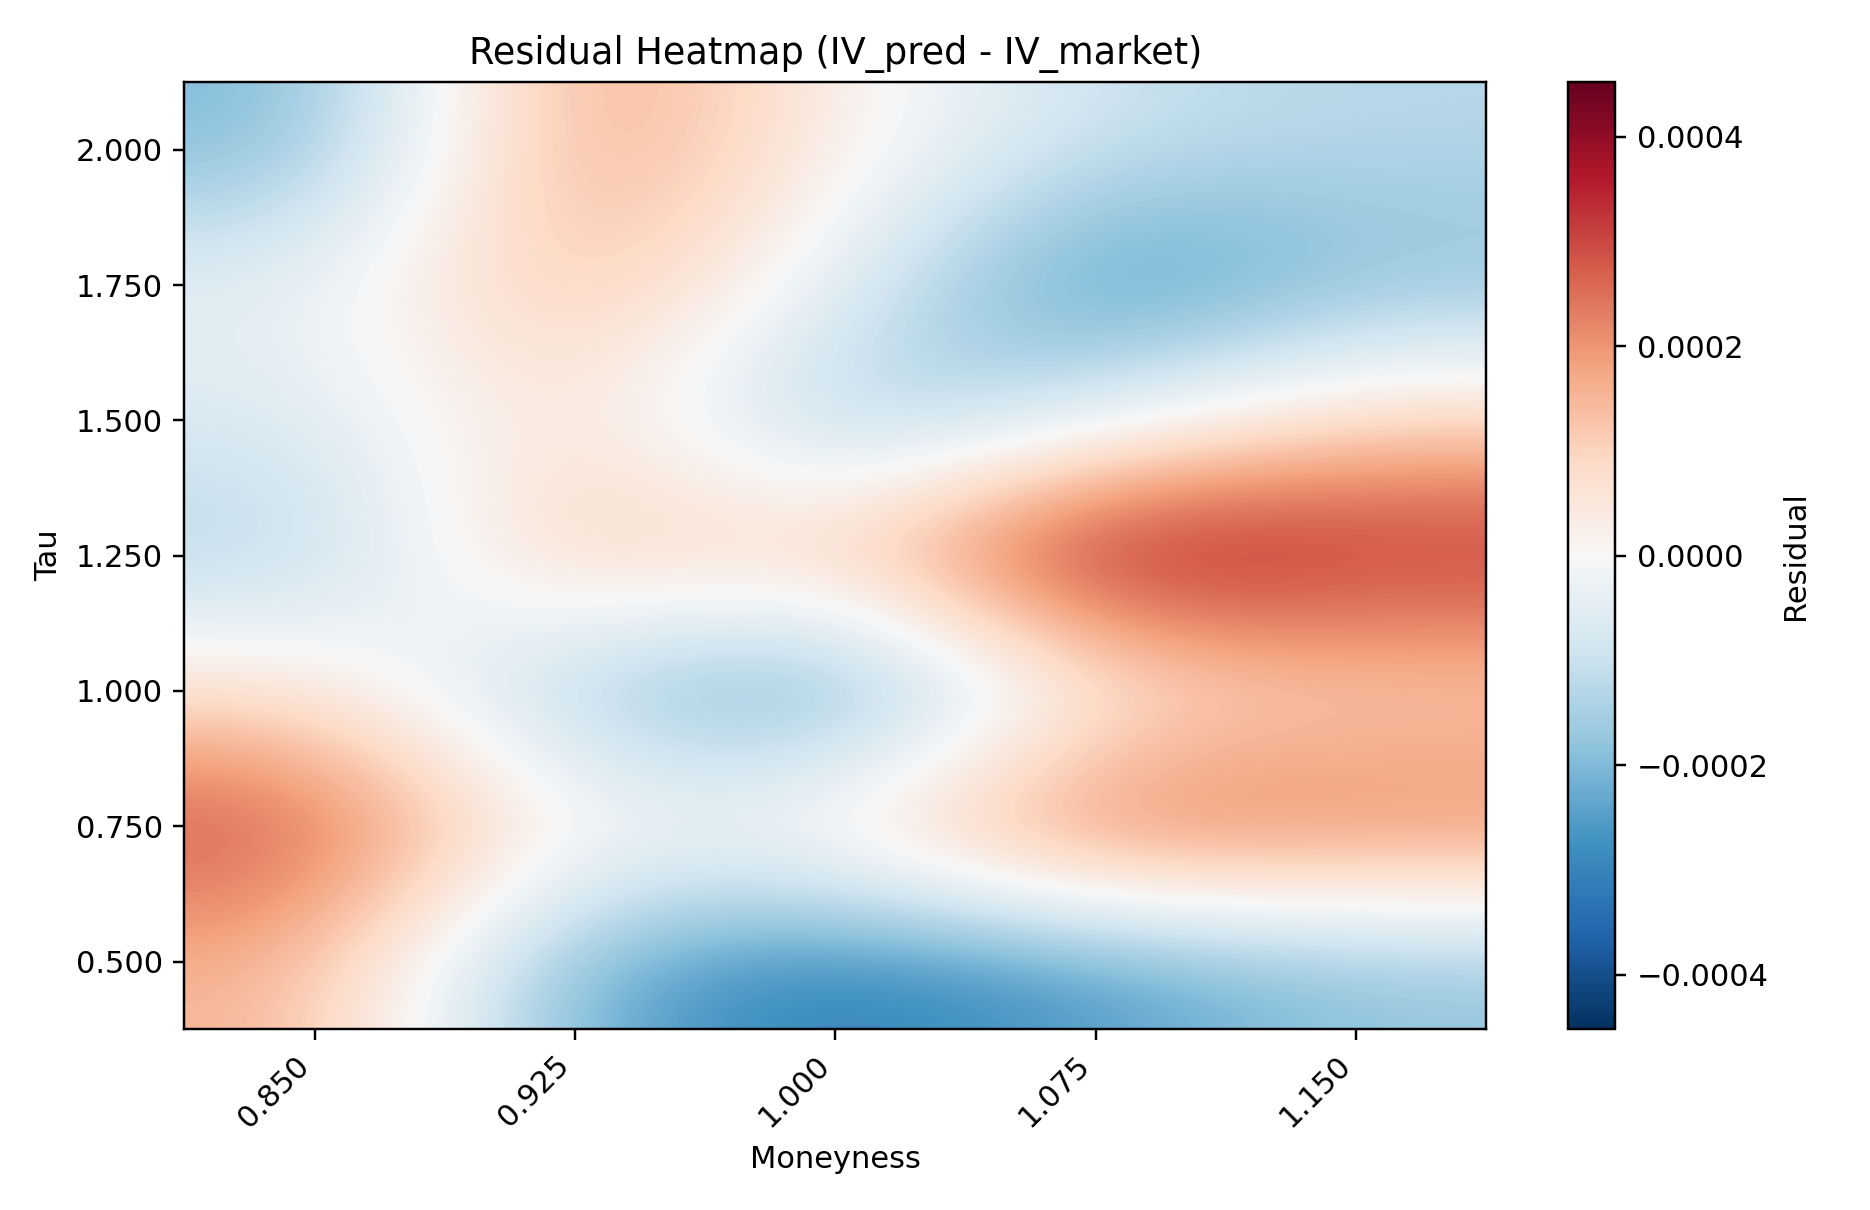
\includegraphics[width=0.86\textwidth]{figures/cann/cann_residual_heatmap_m_tau_no_reg_smooth.png}
    \caption{Signed implied-volatility residual map for the selected CaNN calibration, defined as \(\mathrm{IV}_{\mathrm{pred}}-\mathrm{IV}_{\mathrm{market}}\). The smoothing is visual only; the calibration is performed on the original quote grid.}
    \label{fig:cann_residual_method}
\end{figure}

To study local identifiability, let
\[
e(\theta)=
\begin{bmatrix}
e_1(\theta) & \cdots & e_{N_q}(\theta)
\end{bmatrix}^{\top}
\]
be the residual vector. Ignoring normalization and regularization for readability, the data term can be written as
\[
J_{\mathrm{data}}(\theta)=e(\theta)^{\top}W e(\theta),
\]
where \(W=\mathrm{diag}(w_1,\dots,w_{N_q})\). Around a low-residual optimum, the Hessian is closely related to the Gauss--Newton matrix
\[
H(\theta^\star)\approx 2 J_e(\theta^\star)^{\top}WJ_e(\theta^\star),
\]
where \(J_e\) is the Jacobian of quote residuals with respect to the calibrated parameters.

This approximation gives the diagnostic its interpretation. Large curvature indicates directions in parameter space where the implied-volatility surface reacts strongly. Small curvature indicates flatter directions, where different parameter values can generate similar quote fits. Cross-terms reveal parameter couplings, which are especially relevant in the Heston model because variance level, variance-of-variance, and mean reversion can partially compensate for each other over limited grids.

\begin{figure}[H]
    \centering
    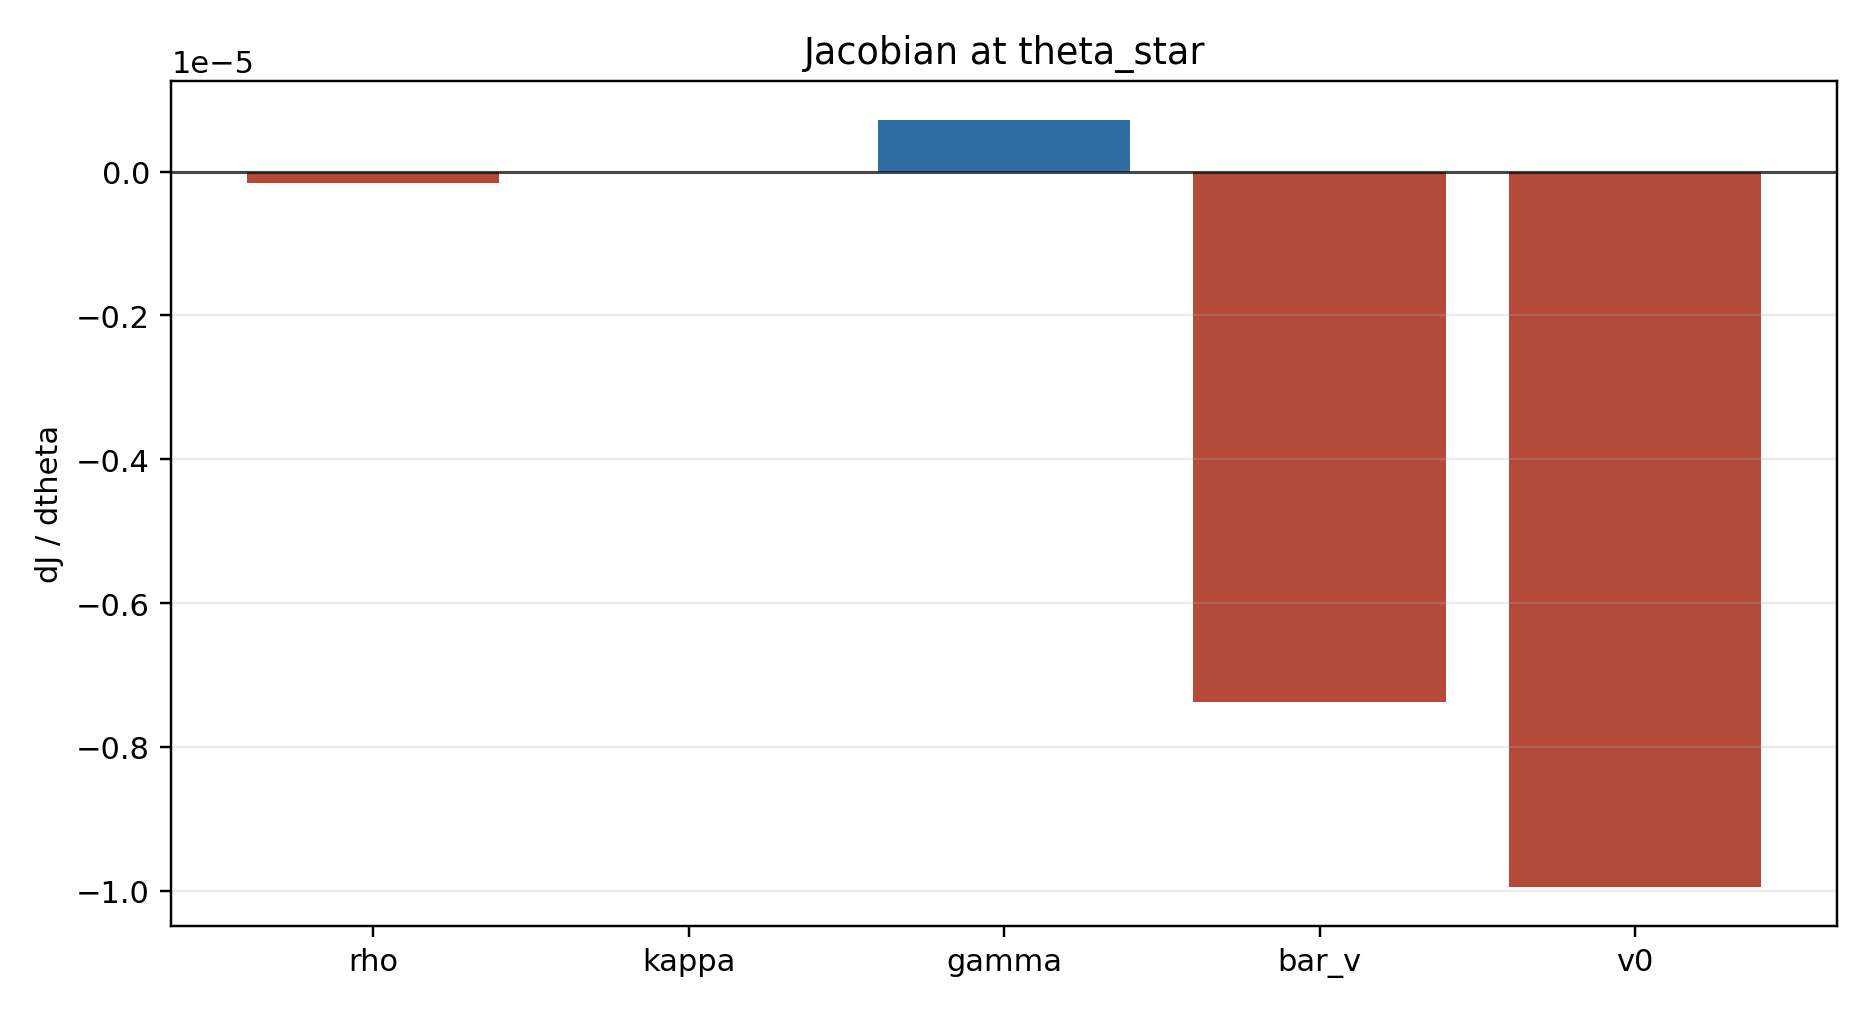
\includegraphics[width=0.72\textwidth]{figures/cann/jacobian_theta_star_no_reg.png}
    \caption{Objective-gradient components at \(\theta^\star\) for the selected no-regularization calibration. Near-zero components support first-order stationarity of the selected solution.}
    \label{fig:cann_jacobian_method}
\end{figure}

\begin{figure}[H]
    \centering
    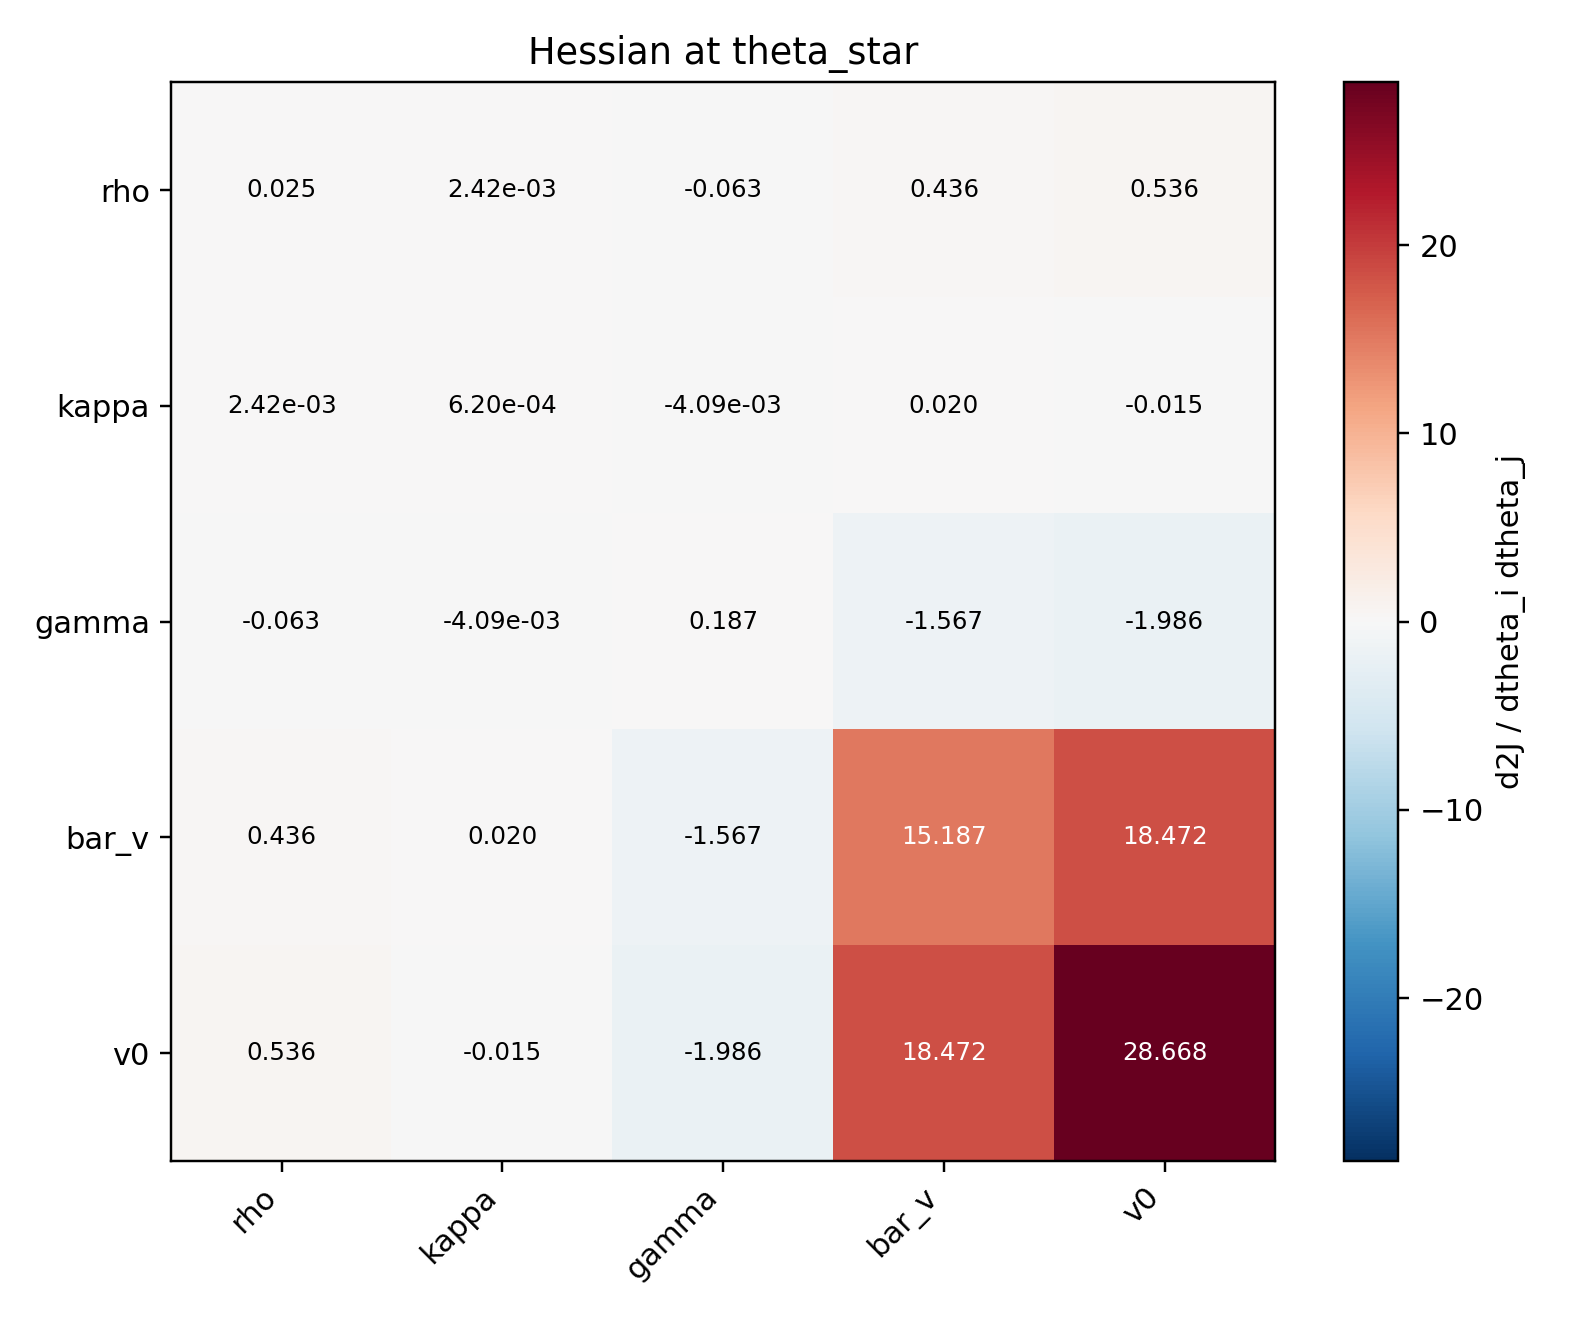
\includegraphics[width=0.78\textwidth]{figures/cann/hessian_theta_star_no_reg.png}
    \caption{Hessian matrix at \(\theta^\star\) for the selected no-regularization calibration. The variance block around \((\bar v,v_0)\) is locally stiffer than the remaining directions, indicating uneven parameter identifiability.}
    \label{fig:cann_hessian_method}
\end{figure}

The resulting reading is deliberately cautious. A small residual map supports the claim that the calibrated vector is market-consistent on the quote grid. A positive local curvature profile supports the claim that the selected solution lies in a stable basin. However, neither observation proves global uniqueness of the Heston inverse problem. The parameter-level conclusions in Chapter~\ref{ch:performance_benchmarks} must therefore be read together with these diagnostics: \((\bar v,v_0)\) are locally more tightly identified in the selected experiment than parameters such as \(\rho\) and \(\gamma\).

%%%%%%%%%%%%%%%%%%%%%%%%%%%%%%%%%%%%%%%%%%%%%%%%%
\section{Interface with the PINN Stage}

The final role of the CaNN stage is to pass a market state to the pricing and Greeks analysis developed later in the thesis. This interface requires a small but important distinction. In calibration, \(v_0^\star\) is one of the inferred Heston parameters. In the PINN formulation, the network is trained over a generic variance state \(v\), while the calibrated value \(v_0^\star\) is inserted only when evaluating the trained model at the current market configuration.

\begin{figure}[H]
    \centering
    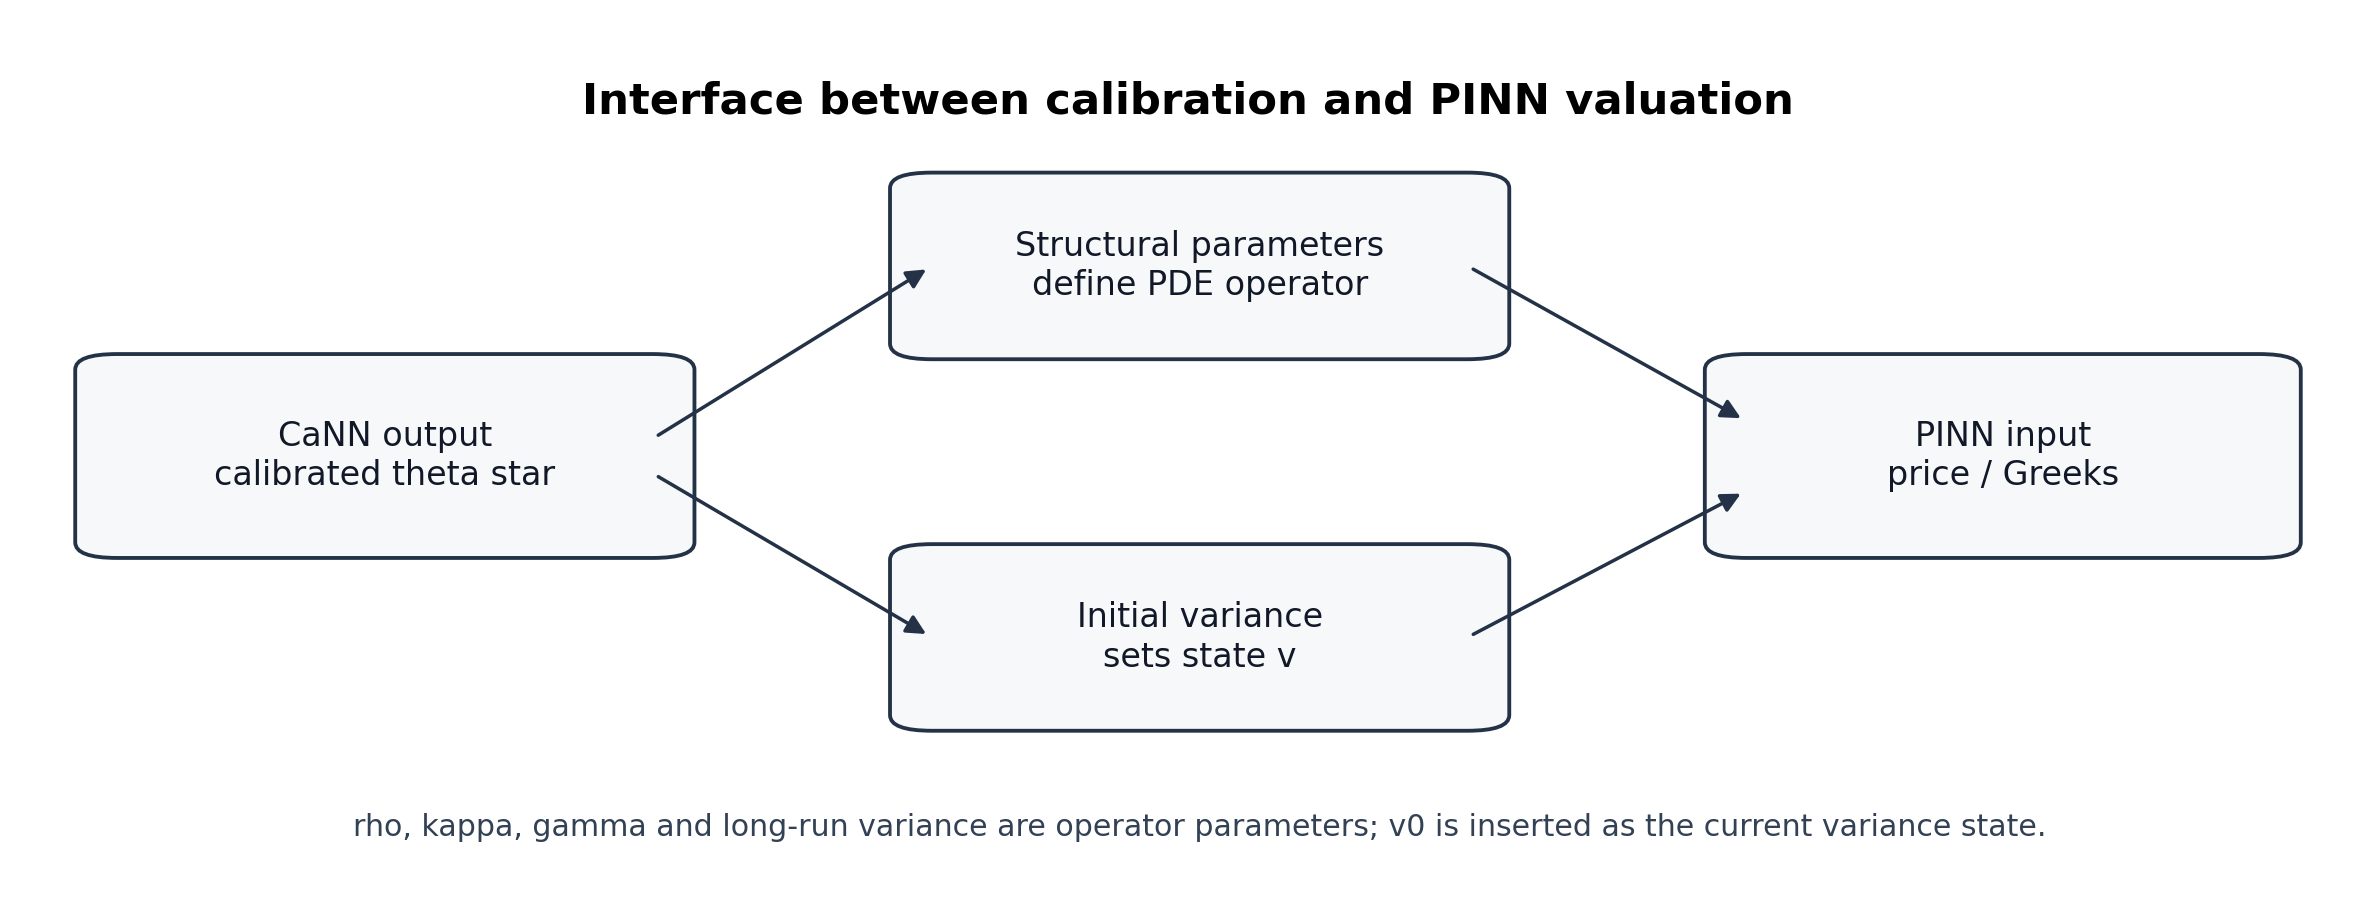
\includegraphics[width=0.88\textwidth]{figures/cann/cann_to_pinn_interface.png}
    \caption{Interface between the calibrated Heston vector and the downstream PINN input convention. Structural parameters define the PDE operator, while \(v_0^\star\) is used as the variance-state coordinate at market evaluation.}
    \label{fig:cann_to_pinn_interface}
\end{figure}

This closes the methodological loop. The ANN pricer makes calibration computationally feasible; the optimizer converts a quote surface into a Heston vector; the diagnostics determine how that vector should be interpreted; and the calibrated state becomes the input configuration for the PINN-based valuation and Greek computation that follows.
